% Created 2021-11-03 Wed 18:55
% Intended LaTeX compiler: pdflatex
\documentclass[11pt]{article}
\usepackage[utf8]{inputenc}
\usepackage[T1]{fontenc}
\usepackage{graphicx}
\usepackage{grffile}
\usepackage{longtable}
\usepackage{wrapfig}
\usepackage{rotating}
\usepackage[normalem]{ulem}
\usepackage{amsmath}
\usepackage{textcomp}
\usepackage{minted}
\usepackage{amssymb}
\usepackage{capt-of}
\usepackage{hyperref}
\date{\today}
\title{}
\hypersetup{
 pdfauthor={},
 pdftitle={},
 pdfkeywords={},
 pdfsubject={},
 pdfcreator={Emacs 27.2 (Org mode 9.4.4)}, 
 pdflang={English}}
\hypersetup{colorlinks, allcolors=., colorlinks=true,linkcolor={blue!78!white}, urlcolor={purple}, filecolor={winered}}

\begin{document}

\tableofcontents
\clearpage
\section{Minha limpeza}
\label{sec:org97358d7}
\subsection{Estado inicial}
\label{sec:orgf56efb0}
\begin{itemize}
\item \texttt{Alcohol} e \texttt{Total.expenditure} têm \textasciitilde{}180 dados faltando (mais da metade dos países e de países diferentes)
\end{itemize}
\begin{verbatim}
    Status      Life.expectancy Adult.Mortality infant.deaths  
Min.   :1.000   Min.   :51.00   Min.   :  1.0   Min.   :  0.0  
1st Qu.:2.000   1st Qu.:65.75   1st Qu.: 74.0   1st Qu.:  0.0  
Median :2.000   Median :73.90   Median :138.0   Median :  2.0  
Mean   :1.825   Mean   :71.62   Mean   :152.9   Mean   : 23.8  
3rd Qu.:2.000   3rd Qu.:76.95   3rd Qu.:213.0   3rd Qu.: 17.0  
Max.   :2.000   Max.   :88.00   Max.   :484.0   Max.   :910.0  

   Alcohol       percentage.expenditure  Hepatitis.B       Measles     
Min.   : 0.010   Min.   :  0.000        Min.   : 6.00   Min.   :    0  
1st Qu.: 2.493   1st Qu.:  0.000        1st Qu.:78.75   1st Qu.:    0  
Median : 5.285   Median :  0.000        Median :93.00   Median :   17  
Mean   : 5.288   Mean   :  2.384        Mean   :82.43   Mean   : 1503  
3rd Qu.: 8.018   3rd Qu.:  0.000        3rd Qu.:97.00   3rd Qu.:  202  
Max.   :10.660   Max.   :364.975        Max.   :99.00   Max.   :90387  
NA's   :177                             NA's   :9                      
     BMI        under.five.deaths     Polio       Total.expenditure
Min.   : 2.50   Min.   :   0.00   Min.   : 5.00   Min.   :6.00     
1st Qu.:24.30   1st Qu.:   0.00   1st Qu.:83.00   1st Qu.:6.54     
Median :48.60   Median :   3.00   Median :93.00   Median :7.08     
Mean   :42.75   Mean   :  31.61   Mean   :83.21   Mean   :7.08     
3rd Qu.:61.40   3rd Qu.:  21.00   3rd Qu.:97.00   3rd Qu.:7.62     
Max.   :77.60   Max.   :1100.00   Max.   :99.00   Max.   :8.16     
NA's   :2                                         NA's   :181      
  Diphtheria       HIV.AIDS           GDP             Population       
Min.   : 6.00   Min.   :0.1000   Min.   :   33.68   Min.   :     2966  
1st Qu.:83.50   1st Qu.:0.1000   1st Qu.:  766.01   1st Qu.:   268071  
Median :93.00   Median :0.1000   Median : 2916.23   Median :  2076086  
Mean   :84.63   Mean   :0.6607   Mean   : 7185.33   Mean   : 11097408  
3rd Qu.:97.00   3rd Qu.:0.4000   3rd Qu.: 7290.11   3rd Qu.:  9940296  
Max.   :99.00   Max.   :9.3000   Max.   :66346.52   Max.   :258162113  
                                 NA's   :29         NA's   :41         
thinness..1.19.years thinness.5.9.years Income.composition.of.resources
Min.   : 0.100       Min.   : 0.100     Min.   :0.3470                 
1st Qu.: 1.500       1st Qu.: 1.500     1st Qu.:0.5650                 
Median : 3.500       Median : 3.400     Median :0.7230                 
Mean   : 4.535       Mean   : 4.576     Mean   :0.6917                 
3rd Qu.: 6.500       3rd Qu.: 6.400     3rd Qu.:0.7980                 
Max.   :26.700       Max.   :27.300     Max.   :0.9480                 
NA's   :2            NA's   :2          NA's   :10                     
  Schooling    
Min.   : 4.90  
1st Qu.:10.80  
Median :13.10  
Mean   :12.93  
3rd Qu.:15.00  
Max.   :20.40  
NA's   :10     
\end{verbatim}

\subsection{Processamento}
\label{sec:orgdd05811}
\begin{itemize}
\item \texttt{Country} e \texttt{Year}
\item Muitos dados faltando: \texttt{Alcohol}, \texttt{Total.expenditure}.
\item Após retirada de ambos, ainda foi feita a retirada dos dados nulos.

\begin{minted}[frame=lines,fontsize=\scriptsize,linenos=false]{r}
life_2015_clean <- na.omit(life_2015_clean) ## eliminando dados nulos
\end{minted}
\end{itemize}

\clearpage
\section{Plot correlação após limpeza dos dados}
\label{sec:orgf491ae7}
\begin{itemize}
\item Dados que possuem pouquíssima correlação com qualquer outros dados:
\begin{itemize}
\item \texttt{percentage.expenditure} (Quantidade gasta em saúde (percentagem do PIB)).
\item \texttt{Measles} (Rubeola).
\item \texttt{Population} (Tamanho da população).
\end{itemize}
\end{itemize}

\href{ein-images/ob-ein-bc5a9463cf1a9262fc216a957d492b0d.png}{\includegraphics[width=.9\linewidth]{/home/buddhilw/PP/MonitoriaEstatistica/ein-images/ob-ein-bc5a9463cf1a9262fc216a957d492b0d.png}}
\clearpage
\section{Plot enviado pelo Jose}
\label{sec:org2df2883}
\begin{itemize}
\item Provável problema:
\begin{itemize}
\item Muitos dados faltando: \texttt{Alcohol}, \texttt{Total.expenditure}.
\end{itemize}
\end{itemize}

\href{img/imagem\_2021-11-03\_174732.png}{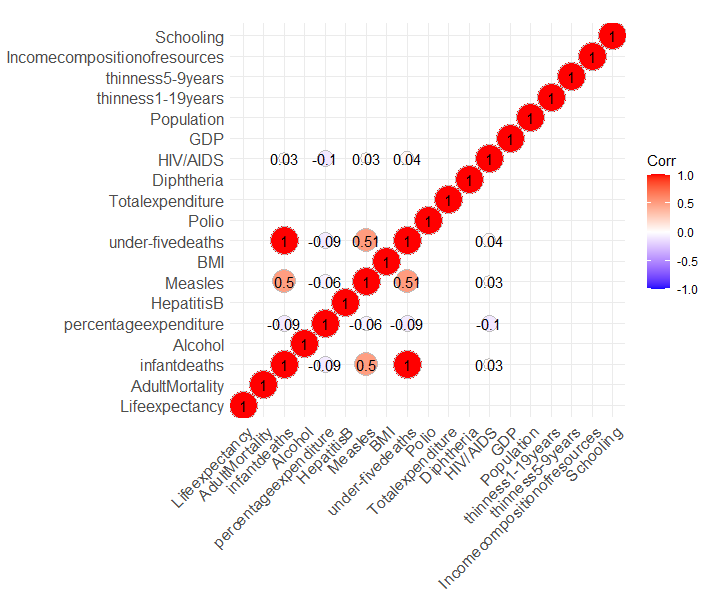
\includegraphics[width=.9\linewidth]{/home/buddhilw/PP/MonitoriaEstatistica/img/imagem_2021-11-03_174732.png}}
\end{document}